\section{Methods}
The chosen datasets are transformed and uploaded to the database where views are created. The data is then used to answer and visualize given questions by plots and maps.


\subsection{Data Integration}
To retrieve the integrated entities from the raw sources, \emph{R} is used as it allows to create data frames that can be pre-analyzed and written to \emph{*.csv}. The R script mostly just readjusts the columns to new frames but also cleans and splits some raw data. Apart from some character level import fixes, the following changes are made to the raw datasets:
\begin{itemize}
\item \textbf{Country}
The country column represents the new \emph{Country} entity. The population columns are split up and added to the new \emph{Population} entity along with country and year. 
\item \textbf{Metal}
Everything but styles represents the new \emph{MetalBand} entity. The styles are split and added to the new \emph{MetalStyle} entity, along with the band name and an autoincrement primary key.
\item \textbf{Terror}
The distinct entries of the location columns form the new \emph{TerrorLocation} entity. These have an ID and are mapped back to the new entity \emph{TerrorEvents}. The up to four weapon types from raw data are organized in the new entity \emph{TerrorWeapon} along with the event ID. The same procedure is applied to up to three attack and target types to yield the new entities \emph{TerrorAttack} and \emph{TerrorWeapon}. The column \emph{related} from raw data is split and added to the new entity \emph{TerrorRelation} along with the event ID and an ID. Finally, for the table \emph{TerrorEvent}, that holds most of the raw data, the columns \emph{year}, \emph{month} \& \emph{day} are combined to a new column \emph{eventDate}.
\item \textbf{Weather}
For each terror location, the closest (< 50km) weather station and then the data for the event dates is retrieved and added to the new \emph{Weather} entity along with the location ID and the weather date.
\end{itemize}
Each entity's file is then uploaded to a \emph{MySQL} database by a \emph{Python} script, using \emph{mysql.connector}, that reads and inserts the rows.

\subsection{Analysis}
The analysis part is written in \emph{Python}, using \emph{matplotlib} to visualize the results. The scripts execute predefined queries, again with the use of \emph{mysql.connector}, plots it and saves the plots in a directory. Three kinds of plots were used:
\begin{itemize}
	\item \textbf{Bar plot} Used for Genre vs Terrorism.
	\item \textbf{Star plot} Used to demonstrate influence of weather on terrorism. The star plot has the advantage of showing changes, in proportions and not only total numbers, nicely. This was achieved by rotating the axes by a certain factor.
	\item \textbf{Graph} Used to compare all other questions. The graphs always shows two lines, one for each aspect that is inspected, to enable a direct comparison between them.
\end{itemize}

Since \emph{MySQL 5.7} doesn't support \emph{LIMIT} in subqueries, a view with the top (most bands) metal countries is created for further analysis. To answer the questions, the following data was gathered:
\begin{itemize}
\item \textbf{Are terror events dependent on the weather?}  For the chosen aspects of terror events (attack type, attack target and use weapon) the significant entries are selected and represented in a star plot. The query matches all events which occurred at the same time and location for which there is weather data available. The result set is then further decreased by selecting only events in the predefined weather condition. The number of events is then counted for each chosen entry.

\item \textbf{Do terror attacks influence founding/splitting of metal bands and vice versa?} 

\item \textbf{Does the population influence the number of existing metal bands?}

\item \textbf{Do terror attacks have an influence on the population?}

\item \textbf{Which main genre has the most terror events?} To get somewhat significant data, the top 30 countries with most (over 15) metal bands are selected. Then the country's main genre is selected along with the number of attacks. Group by genre, sum attacks and mean attacks by countries yields the result.
\end{itemize}



\section{Results}
The posed questions are answered by creating visualizations of the integrated data. Each visualization is designed to show if there is a correlation between the inspected attributes.

\subsection{Are terror events dependent on the weather?}
Here, the influence of the weather on terror events is inspected. The visualizations show the number of events that took place under the specified conditions. The weather influence is measured by observing the distribution of terror events for different conditions.

The weather data contains information about the daily mean temperature and daily precipitation. The temperature is split into intervals of 10$^\circ$C beginning with $< -10^\circ$C and ending with $> 30^\circ$C. The daily precipitation is mapped to types of rain, namely: no rain, light rain, moderate rain, heavy rain and very heavy rain.

For the terror events, three aspects are chosen:
\begin{itemize}
	\item Types of terror attacks
	\item The targets of attacks
	\item The used weapons in the attacks
\end{itemize}

These three aspects are represented by the tables \texttt{TerrorAttack}, \texttt{TerrorTarget} and \texttt{TerrorWeapons}, for which only the most significant attributes are chosen, if the total number of them is too large.

\subsection{Weather - Attack Types}
There are nine distinct attack types, which are all displayed in the visualization. Bombing is the most frequent one for each weather condition, followed by armed assault.

\begin{figure}[!ht]
\centering
    \subfloat[]{\includegraphics[width=.6\textwidth]{Rain-Attack/g2-rain0_starDiagram}}\qquad\\
    \subfloat[]{\includegraphics[width=.29\textwidth]{Rain-Attack/g2-rain01-1_starDiagram}}\qquad
    \subfloat[]{\includegraphics[width=.29\textwidth]{Rain-Attack/g2-rain11-5_starDiagram}}\qquad\\
    \subfloat[]{\includegraphics[width=.29\textwidth]{Rain-Attack/g2-rain51-20_starDiagram}}\qquad
    \subfloat[]{\includegraphics[width=.29\textwidth]{Rain-Attack/g2-rain>201_starDiagram}}
\caption{Influence of rain on terror attack types}
\end{figure}

The influence of rain on attack types is very low, as the different types are proportionally similar for each type of rain.

\newpage

\begin{figure}[!ht]
\centering
    \subfloat[]{\includegraphics[width=.28\textwidth]{Temp-Attack/g2-temp<-100_starDiagram}}\qquad
    \subfloat[]{\includegraphics[width=.29\textwidth]{Temp-Attack/g2-temp-101-0_starDiagram}}\qquad
    \subfloat[]{\includegraphics[width=.29\textwidth]{Temp-Attack/g2-temp1-100_starDiagram}}\qquad
    \subfloat[]{\includegraphics[width=.29\textwidth]{Temp-Attack/g2-temp101-200_starDiagram}}\qquad
    \subfloat[]{\includegraphics[width=.29\textwidth]{Temp-Attack/g2-temp201-300_starDiagram}}\qquad
    \subfloat[]{\includegraphics[width=.29\textwidth]{Temp-Attack/g2-temp>301_starDiagram}}
\caption{Influence of temperature on terror attack types}
\label{fig:example subfigure}
\end{figure}

The temperature has a greater influence on attack types. It can be observed that more armed assaults take place when the temperature rises.

\subsection{Weather - Attack Targets}
The number of distinct target types is quite large, since they can be very specific (e.g. Priest). For the analysis, the ten most representative attributes have been chosen. Different to the attack type, the target types vary more for the different conditions.

\begin{figure}[!ht]
\centering
    \subfloat[]{\includegraphics[width=.6\textwidth]{Rain-Target/g2-rain0_starDiagram}}\qquad\\
    \subfloat[]{\includegraphics[width=.29\textwidth]{Rain-Target/g2-rain01-1_starDiagram}}\qquad
    \subfloat[]{\includegraphics[width=.29\textwidth]{Rain-Target/g2-rain11-5_starDiagram}}\qquad\\
    \subfloat[]{\includegraphics[width=.29\textwidth]{Rain-Target/g2-rain51-20_starDiagram}}\qquad
    \subfloat[]{\includegraphics[width=.29\textwidth]{Rain-Target/g2-rain>201_starDiagram}}
\caption{Influence of rain on attack targets}
\end{figure}

It can be observed, that heavier rain results in a bigger number of attacks on military units, patrols and convoys.


\newpage

\begin{figure}[!ht]
\centering
    \subfloat[]{\includegraphics[width=.28\textwidth]{Temp-Target/g2-temp<-100_starDiagram}}\qquad
    \subfloat[]{\includegraphics[width=.29\textwidth]{Temp-Target/g2-temp-101-0_starDiagram}}\qquad
    \subfloat[]{\includegraphics[width=.29\textwidth]{Temp-Target/g2-temp1-100_starDiagram}}\qquad
    \subfloat[]{\includegraphics[width=.29\textwidth]{Temp-Target/g2-temp101-200_starDiagram}}\qquad
    \subfloat[]{\includegraphics[width=.29\textwidth]{Temp-Target/g2-temp201-300_starDiagram}}\qquad
    \subfloat[]{\includegraphics[width=.29\textwidth]{Temp-Target/g2-temp>301_starDiagram}}
\caption{Influence of temperature on attack targets}
\label{fig:example subfigure}
\end{figure}

Lower temperatures have a high number of attacks on military personnel. With increasing temperature, this shifts towards civilians. Therefore, with higher temperature, more civilians but less military personnel are attacked. 

\subsection{Weather - Attack Weapon}
There are, like attack targets, many distinct attack weapons. Again, the ten most representative attributes have been chosen. The weapons have a high correlation to the attack types, seen by the attributes \texttt{Bombing/Explosion \& Unknown explosive type} and \texttt{Armed assault \& Unknown gun type}.

\begin{figure}[!ht]
\centering
    \subfloat[]{\includegraphics[width=.6\textwidth]{Rain-Weapon/g2-rain0_starDiagram}}\qquad\\
    \subfloat[]{\includegraphics[width=.29\textwidth]{Rain-Weapon/g2-rain01-1_starDiagram}}\qquad
    \subfloat[]{\includegraphics[width=.29\textwidth]{Rain-Weapon/g2-rain11-5_starDiagram}}\qquad\\
    \subfloat[]{\includegraphics[width=.29\textwidth]{Rain-Weapon/g2-rain51-20_starDiagram}}\qquad
    \subfloat[]{\includegraphics[width=.29\textwidth]{Rain-Weapon/g2-rain>201_starDiagram}}
\caption{Influence of rain on terror attack weapons}
\end{figure}

Similar to the attack types, the influence of rain  on the used weapons can hardly be seen.


\begin{figure}[!ht]
\centering
    \subfloat[]{\includegraphics[width=.28\textwidth]{Temp-Weapon/g2-temp<-100_starDiagram}}\qquad
    \subfloat[]{\includegraphics[width=.29\textwidth]{Temp-Weapon/g2-temp-101-0_starDiagram}}\qquad
    \subfloat[]{\includegraphics[width=.29\textwidth]{Temp-Weapon/g2-temp1-100_starDiagram}}\qquad
    \subfloat[]{\includegraphics[width=.29\textwidth]{Temp-Weapon/g2-temp101-200_starDiagram}}\qquad
    \subfloat[]{\includegraphics[width=.29\textwidth]{Temp-Weapon/g2-temp201-300_starDiagram}}\qquad
    \subfloat[]{\includegraphics[width=.29\textwidth]{Temp-Weapon/g2-temp>301_starDiagram}}
\caption{Influence of temperature on terror attack weapons}
\label{fig:example subfigure}
\end{figure}

As the armed assaults increase with temperature, the number of guns used increases as well.





% TERROR VS NR OF METAL BANDS
\subsection{Terrorism vs number of metal bands}
Are acts of terrorism related to the number of metal bands? These plots show the number of formed, split and existing metalbands vs the number of attacks per year.
\begin{figure}[hbt!]
	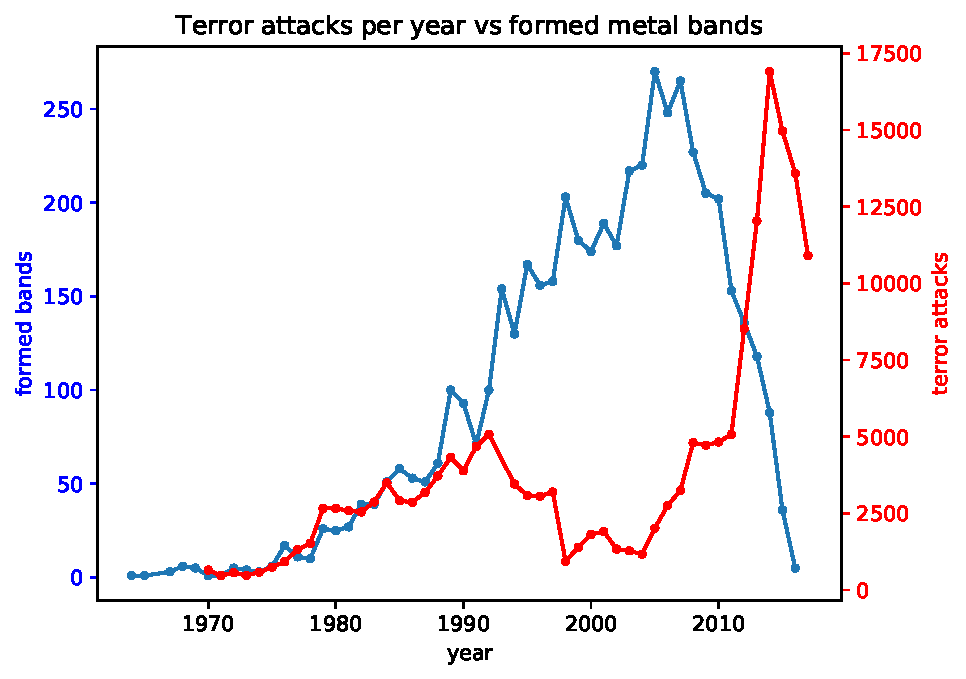
\includegraphics[width=0.3\textwidth]{Band-Terror/g2-attacksVsBandsFormed}
	\centering
	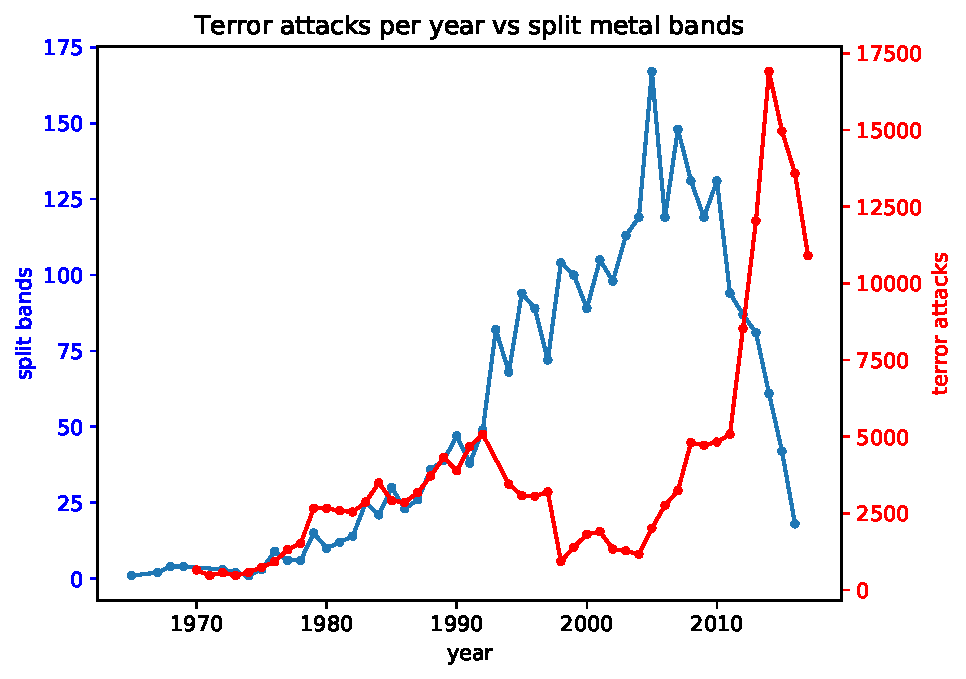
\includegraphics[width=0.3\textwidth]{Band-Terror/g2-attacksVsBandsSplit}
	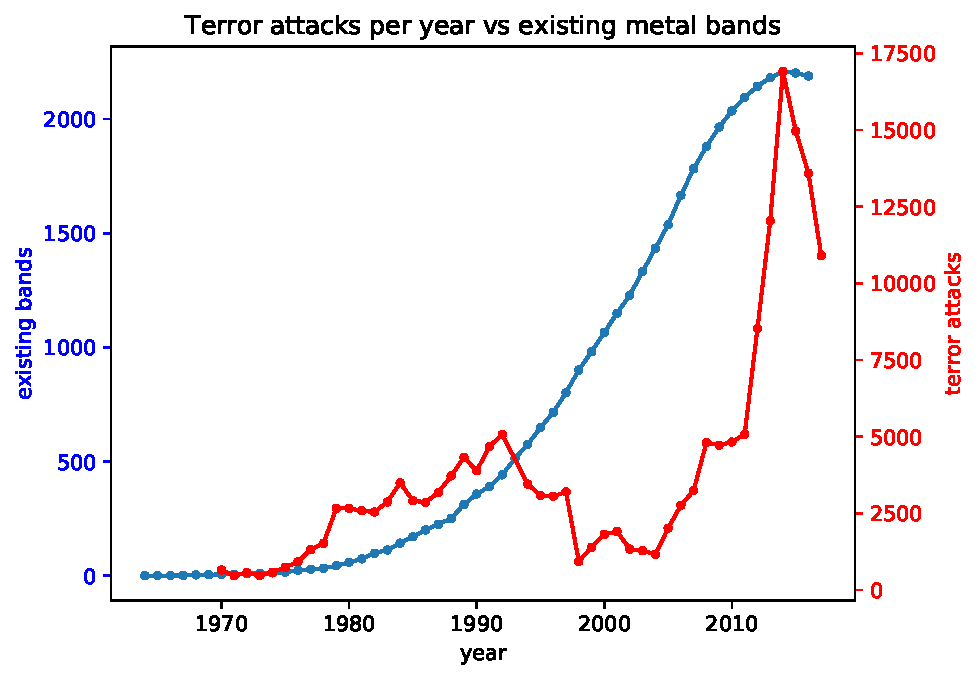
\includegraphics[width=0.3\textwidth]{Band-Terror/g2-attacksVsBandsExisting}
	\caption{formed, split and existing | l,blue: bands / r,red: attacks}
\end{figure}
The curves of formed and split metal bands show the same evolution. First the data is aligned, then it diverges. To have another view, the mean data (existing bands) was also plotted. One could say that terrorism triggered the creation of metal, but then metal went all in. A peak of terrorism then stopped the rapid growth. But no, the number of terror attacks is probably not related to the number of metal bands.


% POPULATION VS NR OF METAL BANDS
\subsection{Population vs number of metal bands}
Is population growth related to number of metal bands? To answer this question, a country's population was plotted against the number of existing metal bands in this country.
\begin{figure}[ht!]
	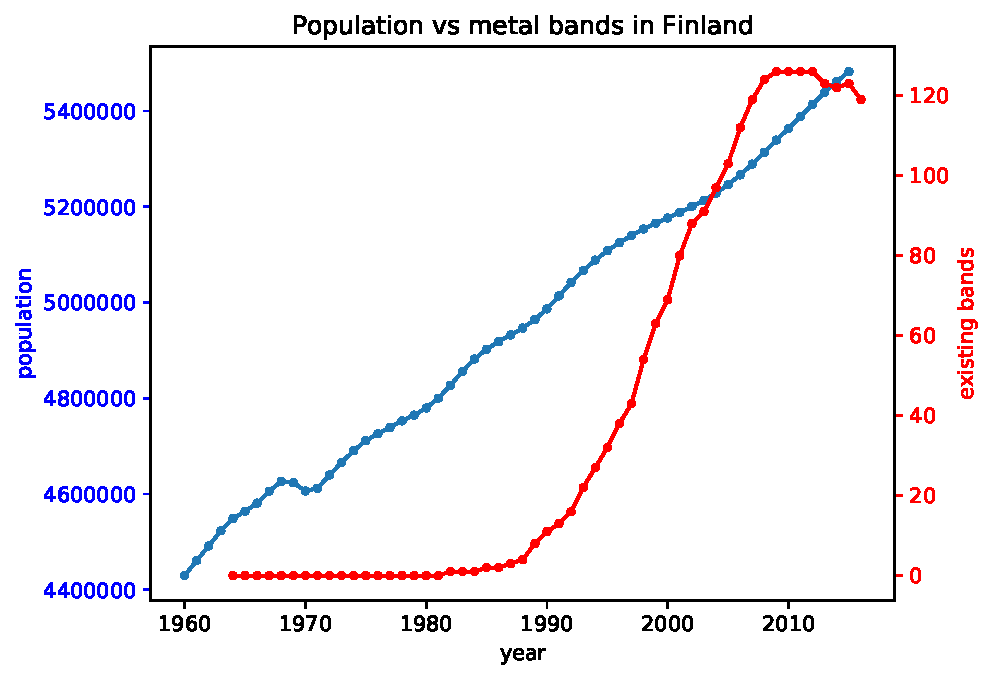
\includegraphics[width=0.3\textwidth]{Population-Bands/g2-populationVsBandFinland}
	\centering
	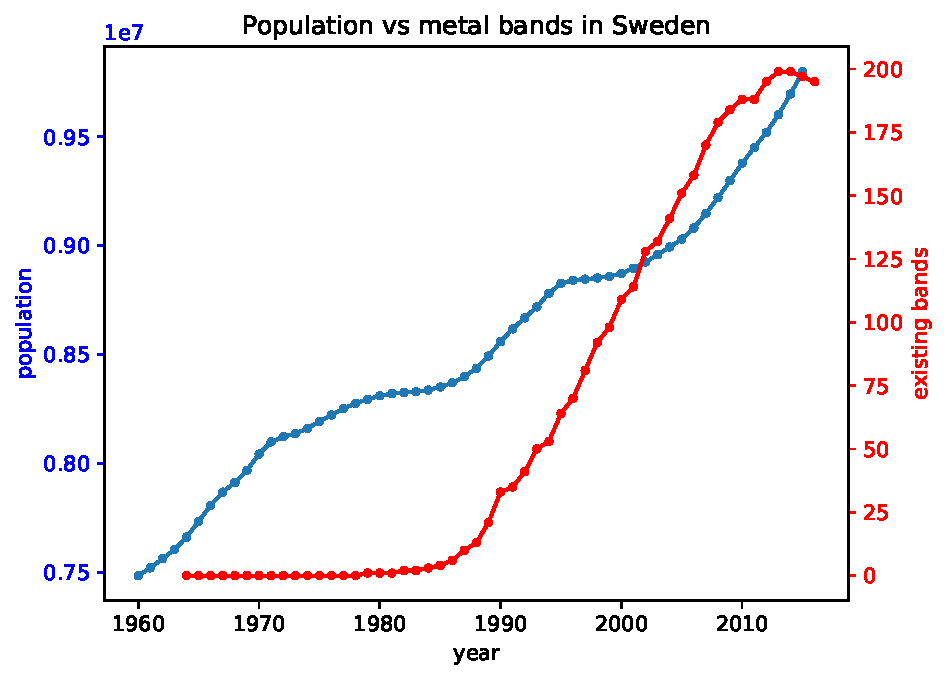
\includegraphics[width=0.3\textwidth]{Population-Bands/g2-populationVsBandSweden}
	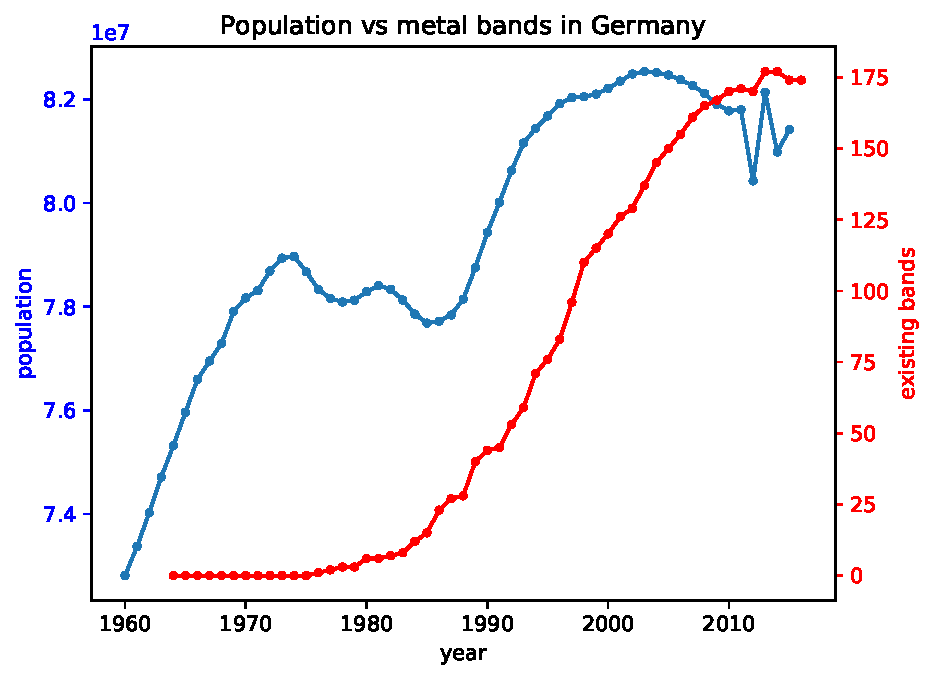
\includegraphics[width=0.3\textwidth]{Population-Bands/g2-populationVsBandGermany}
	\caption{Finland, Sweden and Germany | l,blue: population / r,red: bands}
\end{figure}
There was a lot of different patterns for population, while the band curve pretty much remains the same, but no interesting correlation. What was found, though, were countries that show an opposite behaviour for population and metal bands.
\begin{figure}[hbt!]
	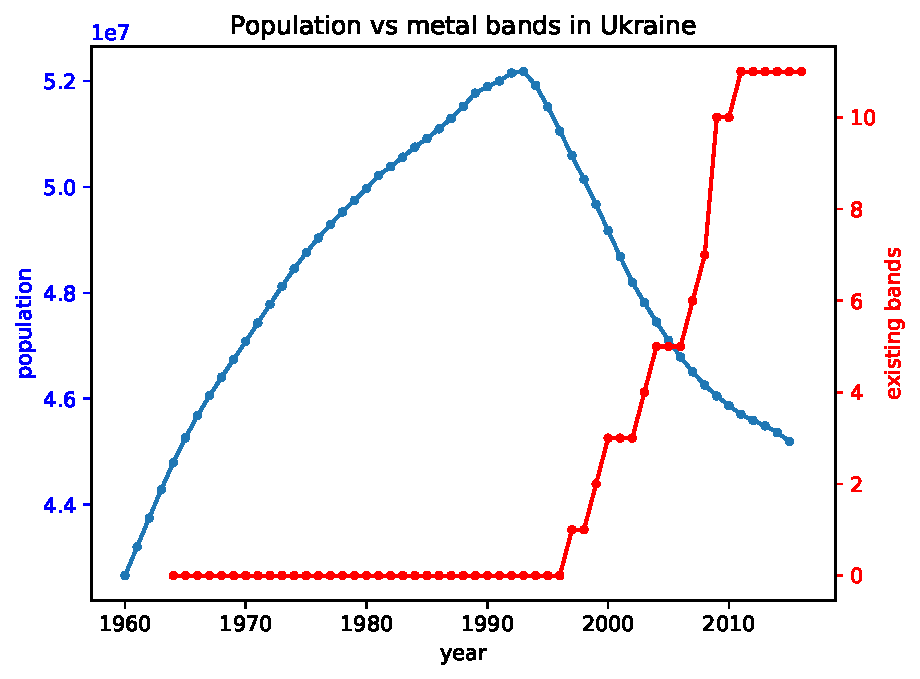
\includegraphics[width=0.3\textwidth]{Population-Bands/g2-populationVsBandUkraine}
	\centering
	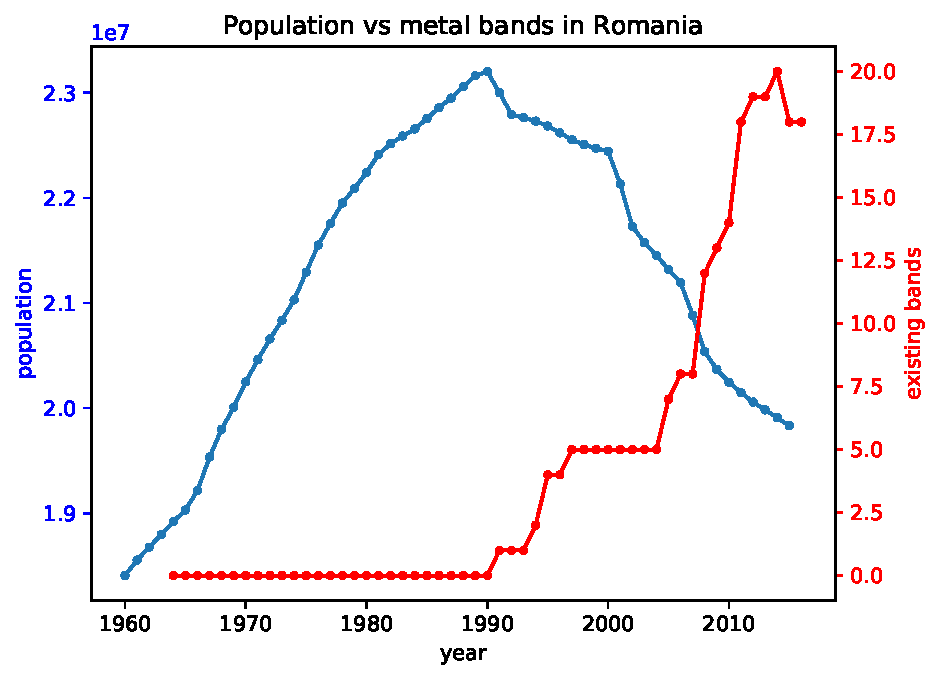
\includegraphics[width=0.3\textwidth]{Population-Bands/g2-populationVsBandRomania}
	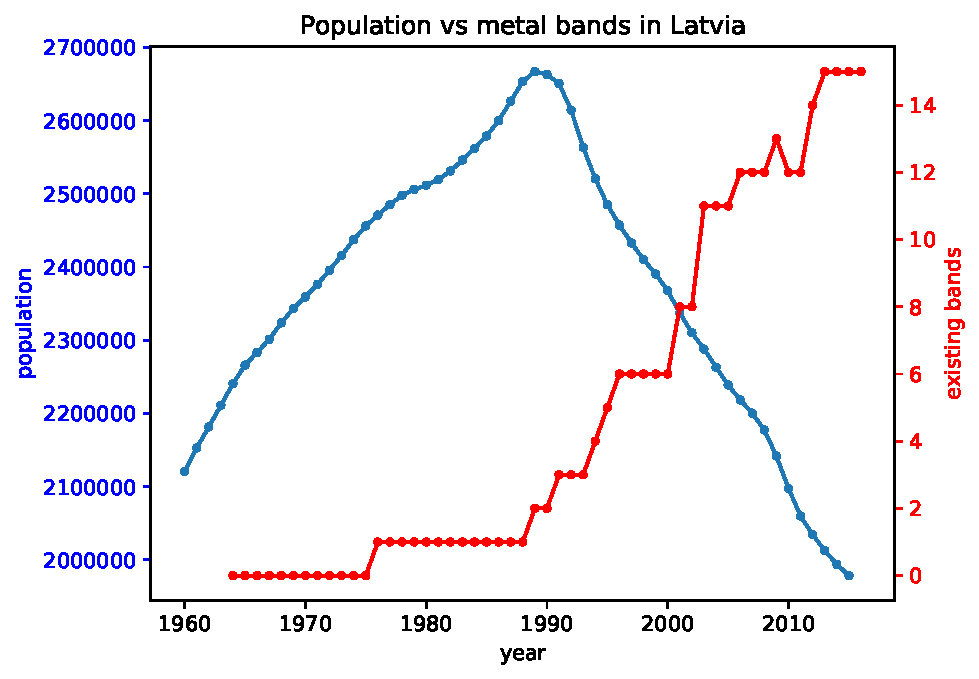
\includegraphics[width=0.3\textwidth]{Population-Bands/g2-populationVsBandLatvia}
	\caption{Ukraine, Romania and Latvia | l,blue: population / r,red: bands}
\end{figure}
It seems as after the rise of metal the population crashed. As it turned out, after opening the borders, due to the fall of communism, there was a lot of emmigration. So population growth and metal bands propably aren't related either.

% TERROR VS POPULATION
\subsection{Terrorism vs population}
Are acts or terror related to population? The number of terror attacks are plotted against the population by country.
\begin{figure}[hbt!]
	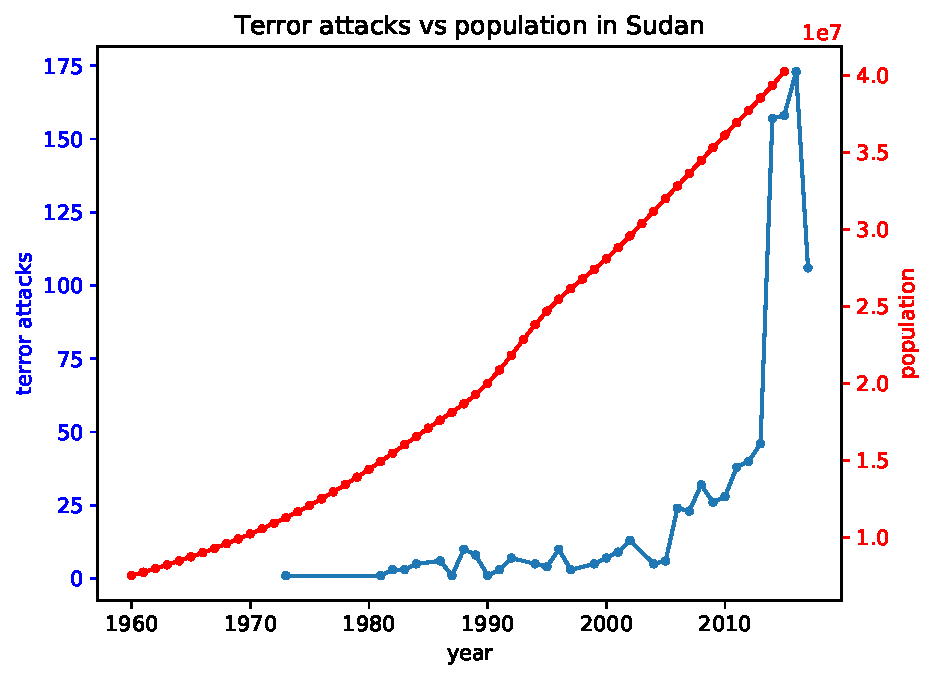
\includegraphics[width=0.3\textwidth]{Population-Terror/g2-attackVsPopulationSudan}
	\centering
	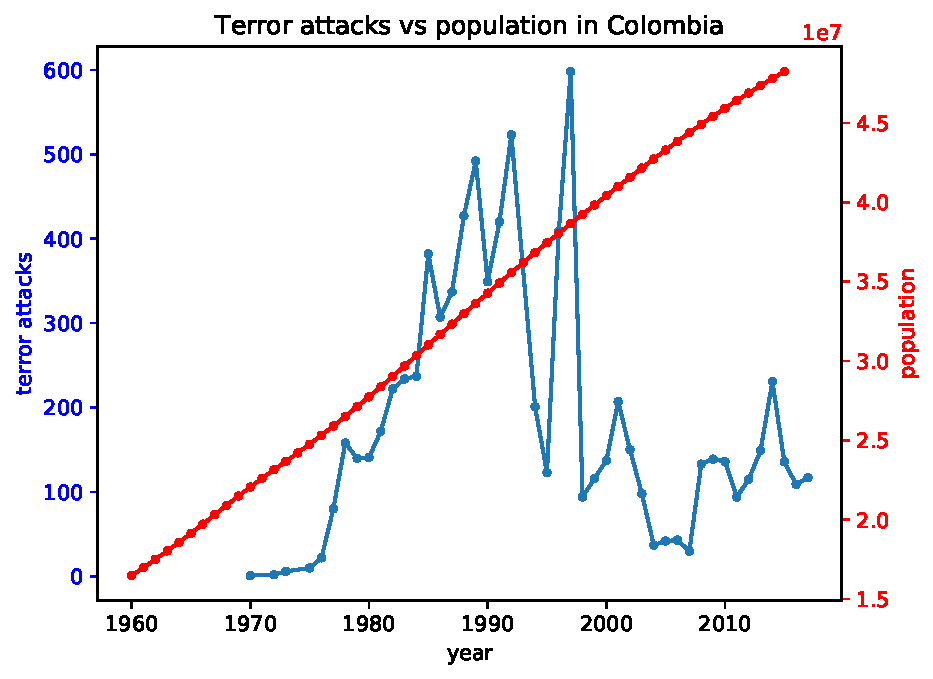
\includegraphics[width=0.3\textwidth]{Population-Terror/g2-attackVsPopulationColombia}
	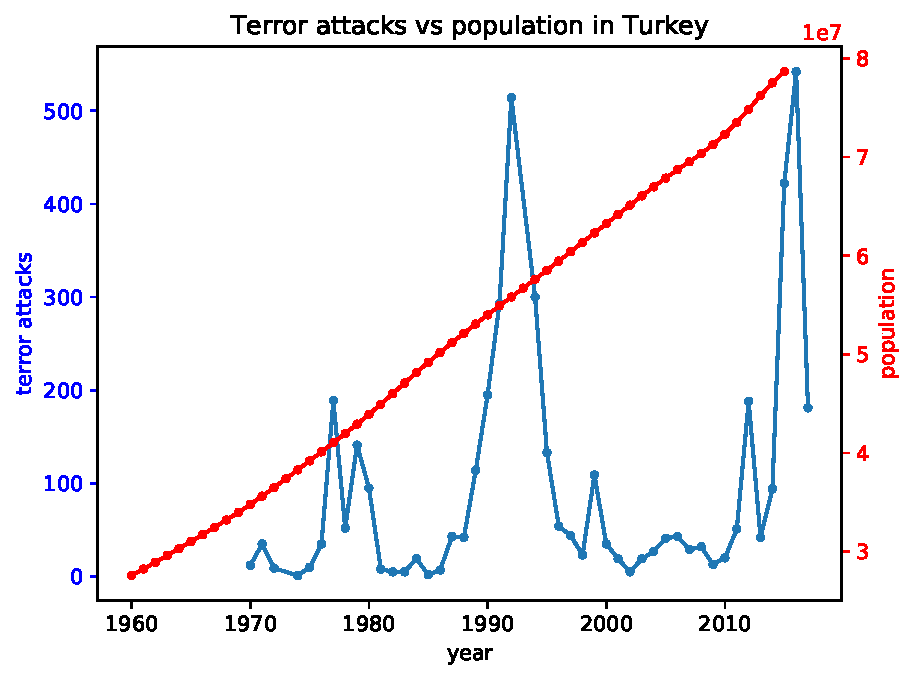
\includegraphics[width=0.3\textwidth]{Population-Terror/g2-attackVsPopulationTurkey}
	\caption{Sudan, Colombia and Turkey l,blue: population / r,red: attacks}
\end{figure}
Obviously population (growth) doesn't care about terror attacks. A lot of different patterns were found, both for population and terrorism. So terrorism and population probably aren't related either, although some countries show interesting figures.
\begin{figure}[hbt!]
	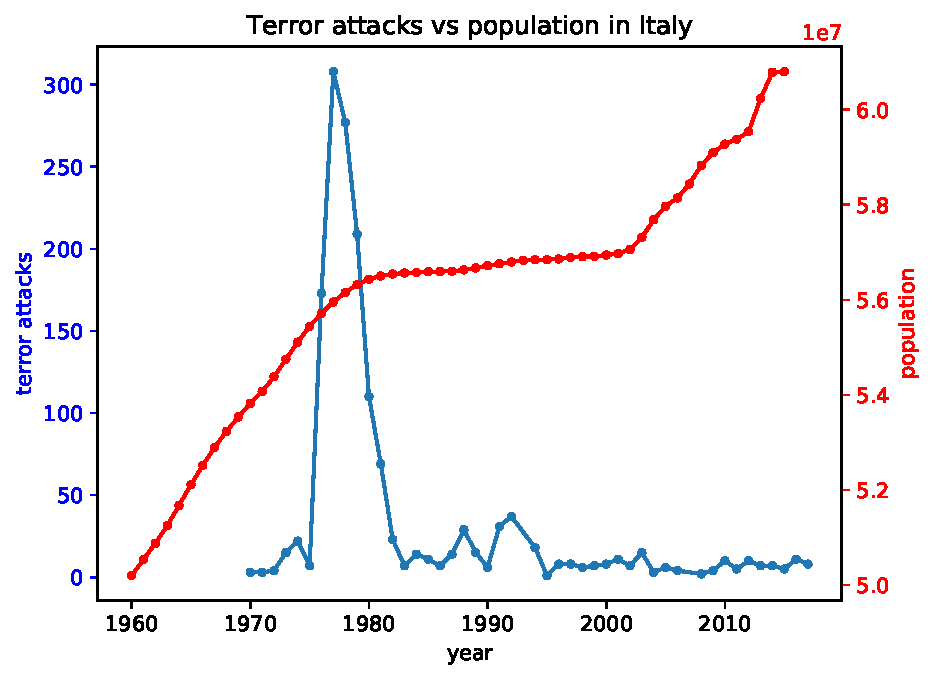
\includegraphics[width=0.3\textwidth]{Population-Terror/g2-attackVsPopulationItaly}
	\centering
	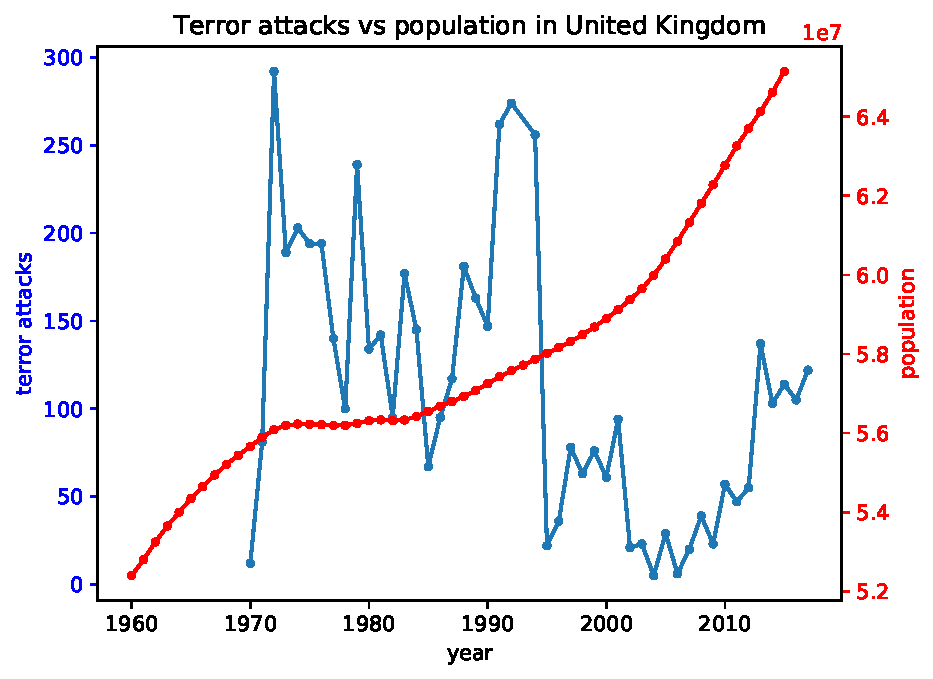
\includegraphics[width=0.3\textwidth]{Population-Terror/g2-attackVsPopulationUnitedKingdom}
	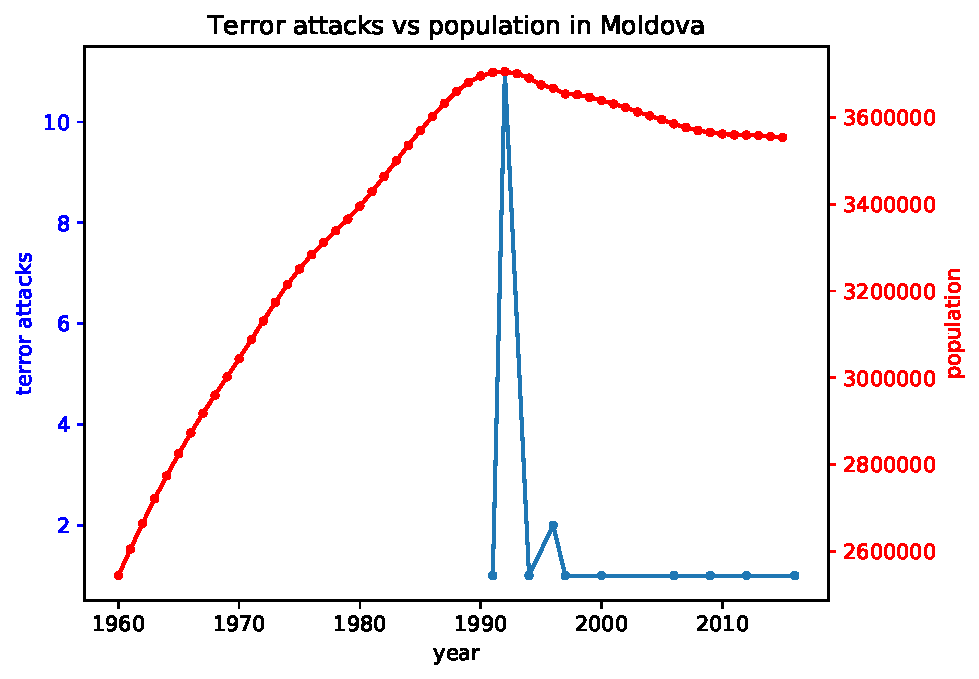
\includegraphics[width=0.3\textwidth]{Population-Terror/g2-attackVsPopulationMoldova}
	\caption{Italy, United Kingdom and Moldova l,blue: population / r,red: attacks}
\end{figure}
Some countries have a stagnating or even decreasing population after or during the presence of terrorism. Moldova is probably also communism related, the behaviour in Italy and the UK remain unknown to the authors.


% GENRE VS ATTACKS
\subsection{A country's main genre vs terror attacks}
Does a country's main (most represented) metal genre have influence on terror?
How do you compare metal genre with terrorism? Comparing band names with types and subtypes of attacks, targets and weapons brought two results: The is a metal band and a terror group called \emph{Condor} and there is a metal band called \emph{Suffocation}, which may or may not be related to 17 incidents in the past years. Number of attacks vs main genre gives us:
\begin{figure}[hbt!]
	\centering
	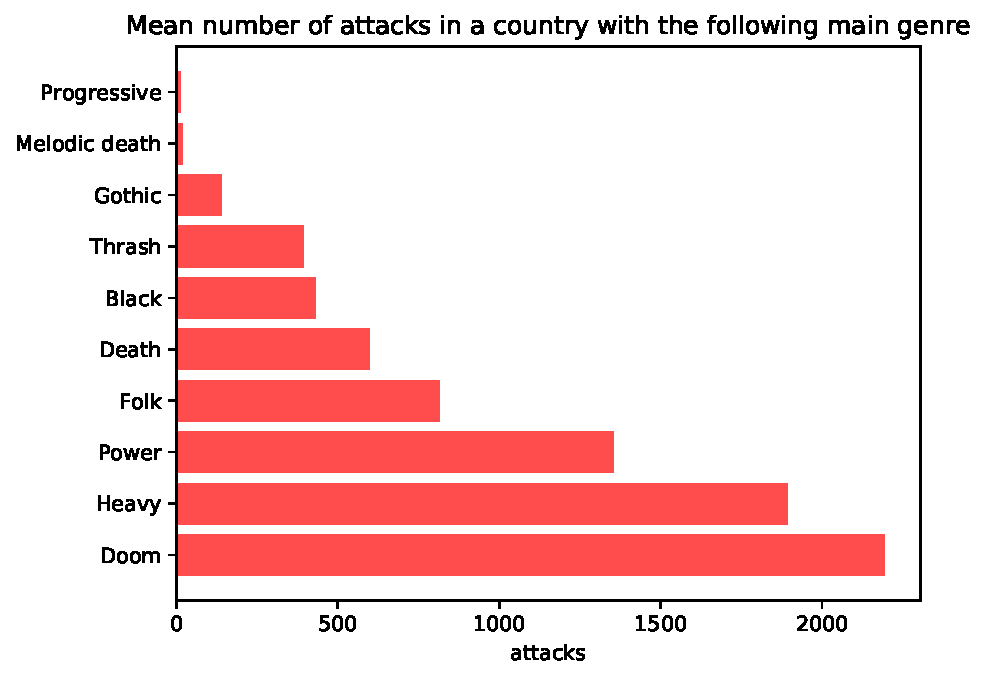
\includegraphics[width=\textwidth]{g2-genreVsTerrorism}
	\caption{Main genre vs terrorism}
\end{figure}
So if your country's main genre is progressive you should be good, if it is doom you should probably leave.


% MAP
\subsection{Terror Map}

\begin{figure}[hbt!]
	\centering
	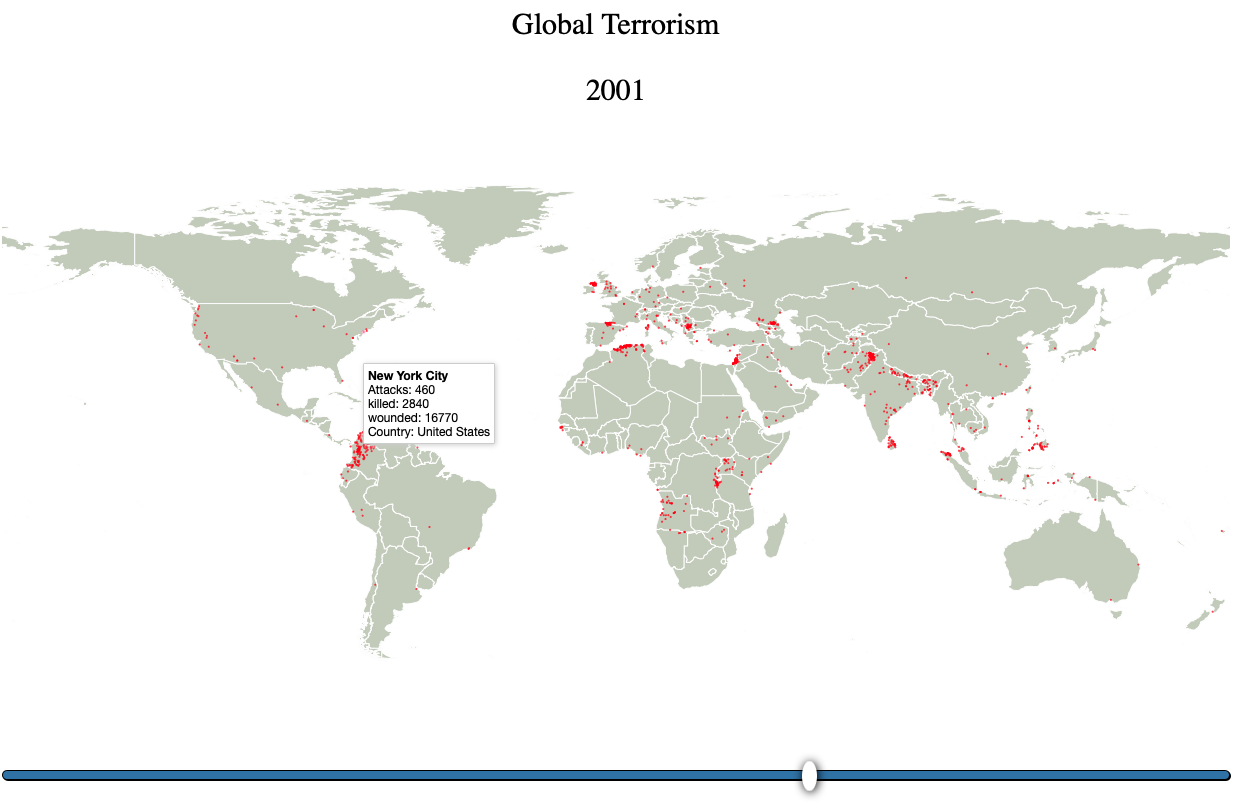
\includegraphics[width=\textwidth]{g2-911.png}
	\caption{Global Terror Map}
\end{figure}
The terror data points were visualized with datamaps. For each year, the distinct locations were retrieved and plotted. Mouseover the location shows the city, country, number of attacks and the number of killed and wounded people.